\documentclass[12pt, block=fill]{beamer}
\usepackage{graphicx}
\usepackage[sfdefault]{FiraSans}
\usepackage{FiraMono}
\usepackage[T1]{fontenc}
\usepackage{xcolor}
\usepackage{mathtools}
\usepackage{txfonts}
\usepackage{ulem}


\usepackage{hyperref}

\definecolor{burntOrange}{rgb}{.8, .5, .1}
\definecolor{textgray}{rgb}{.8,.8,.8}
\definecolor{berkeleyYellow}{HTML}{FDB515}

\usetheme[
titleformat frame = smallcaps,
subsectionpage = progressbar]
{metropolis}

\metroset{
  block=fill
}

\usepackage{pgfpages}
\setbeameroption{hide notes} % Only slides
% \setbeameroption{show only notes} % Only notes
  % \setbeameroption{show notes on second screen=right} % Both
\setbeamerfont{note page}{size=\footnotesize}

\newcommand{\E}{\text{E}}
\newcommand{\V}{\text{V}}
\newcommand{\cov}{\text{cov}}
\newcommand{\bs}{\boldsymbol}

\newcommand{\Z}{\mathbb{Z}}
\newcommand{\R}{\mathbb{R}}
\newcommand{\N}{\mathbb{N}}
\newcommand{\paul}[1]{{\color{red}#1}}
\newcommand{\alex}[1]{\textcolor{berkeleyYellow}{#1}}


\title{Week 4}
\subtitle{Conditional Expectation and the Best Linear Predictor}

\author{Paul Laskowski and Alex Hughes}
\institute{UC Berkeley, School of Information}

\begin{document}

\begin{frame}
  \maketitle
\end{frame}

\section{Motivating Examples}

\begin{frame}
  \frametitle{Motivating Examples}

  Given a random variable \textbf{X} and another random variable
  \textbf{Y}, you often want to make predictions about \textbf{Y} that
  are \textit{as good as possible.}

  \note[item]{This is the goal of a \textit{ton} of what we want to
    accomplish in supervised, structured data learning tasks! We
    aren't going to get all the way there, but we're going to build
    the foundations for how we understand this task this week.}

  \begin{itemize}
  \item Given some budget, what will an organization's head count be
    next year?
  \item Given a citizen's age and income, how likely are they to vote?
  \item Given a set of sounds picked up by a microphone, what are the
    chances that someone in the room has fallen down (Sound Flux,
    2019)?
  \item Given a set of voxels, does an image contain a malignant
    tumor?
  \end{itemize}

  \note[item]{As you may have guessed, we're not just going to head
    straight to making predictions. We're going to built on top of
    things that you already know from the last two weeks, and we're
    going to derive new tools to use that we can \textit{know} will
    work.}
  
\end{frame}

\begin{frame}
  \frametitle{Plan for the Week}
  Two sections: 
  \begin{enumerate}
  \item Conditional expectations 
  \item Best predictors and best linear predictors
  \end{enumerate}

  \note[item]{First, we'll practice working with covariance and
    correlation - these are the most foundational math tools that
    we'll need to work with joint distributions.}
  \note[item]{Next, we'll study conditional expectation - this is
    an important way of summarizing the information in a joint
    distribution. We can ask, what is the shape of the data, provided
    that \textit{some other thing} has occurred.} 
  \note[item]{Finally, we'll figure out how to make predictions
    for one random variable, given another - a very important task for
    data scientists.}
\end{frame}

\begin{frame}
  \frametitle{Plan for the Week (cont.)}
  At the end of this week, you will be able to:
  \begin{itemize}
  \item Derive statements describing relationships among random variables
  \item Understand how to divide variance into a part that is explained and an error component that you have not explained
  \item Understand how a best linear predictor uses information
      from a set of random variables to help us predict the value of
      an outcome
    
    \note[item]{At the end of this week, you'll understand how variation
      in a set of random variables can be used to explain variation in
      another random variable.  This is at the very heart of models for
      linear regression.} 
    \note[item]{Our goal throughout this part of the presentation is to
      work with the foundations of the math, rather than the specifics
      of \textit{one particular} integration. We'll do plenty of math in
      the course, but we're trying to target your effirts.} 
    \note[item]{To do this, we're going to try rely on stand-in
      random variables -- $X \& Y$ -- that \textit{could} be any
      arbitrary function.}
    \note[item]{This lets us engage with the concepts -- which are
      challenging -- without sitting and working pencil-and-paper on
      cranking through the math.}
    \note[item]{There is a general principle here that we'd like you to
      start to learn -- it is exceedingly difficult to work at a
      conceptual level \textbf{and} a fingers-to-the keyboards level at
      the same time.} 
    \note[item]{At times, we're going to illustrate these 
      points by coding. Now, a few words about this -- many of the
      theorems that we prove have sample analogues (this is an applied
      class -- and we're going to get to this in the next unit.) We may
      show you the sample version to help build intuition, but your
      main job in these weeks is to practice with random variables.
      Use the sample to build intuition but then go and make sure you
      understand the proof for random variables.}  
  \end{itemize}
\end{frame}

\section{Conditional Expectation}
\section{Introduction to Conditional Expectation}

\begin{frame}
  \frametitle{Introduction to Conditional Expectation, Part I}
  To this point, we have characterized random variables with three
  concepts:
  \begin{enumerate}
  \item \textbf{The Expected Value}, $\E[X]$
  \item \textbf{The Variance}, $\V[X]$
  \item\textbf{The Covariance}, $\cov[X,Y]$
  \end{enumerate}
  But, when there is dependence between two random variables $X$ and
  $Y$, then if we know something about $X$, we might be able to make a
  new contextualized statement about the \textit{conditional
    distribution}. \\
  \note[item]{We've seen how to use expectation and var to summarize a
    distribution, but we've also seen how observing one variable lets
    us define a conditional distribution on another variable.  Now
    it's time to put those two concepts together.}  \note[item]{We've
    got the Frostee. We've got the fries. Let's do this.}
\end{frame}

\begin{frame}
  \frametitle{Introduction to Conditional Expectation, Part II}
  We began the week with the questions:
  \begin{itemize}
  \item Given some budget, what will an organization's head count be
    next year?
  \item Given some attributes about a citizen, how likely are they to
    vote?
  \item Given a set of sounds picked up by a microphone, what are the
    chances that someone in the room has fallen down (Sound Flux,
    2019)?
  \item Given a set of voxels, does this image contain a malignant
    tumor?
  \end{itemize}
\end{frame}

\begin{frame}
  \frametitle{Introduction to Conditional Expectation, Part III}
  But, those were all conditional statements!  \note[item]{Conditional
    statements let us update general knowledge to make more specific,
    \textit{better} (in terms of MSE) statements.}
 
  Rather than saying, ``On average, 78\% of the electorate votes in
  any given election,'' we can instead say:

  \begin{itemize}
  \item ``Among people 29 or younger, 41\% voted in the last
    presidential election''
  \item ``Among people who \textit{have} voted before, 90\% will vote
    in any given election''
  \end{itemize}

  \note[item]{It is way lower in off-cycle elections -- about 30\% of
    people younger than 29 vote in these elections.}
  \note[item]{Because there is a probability distribution across these
    two mutually exclusive cases, we could actually figure out what
    the population prevalence of these two types are.}  This is our
  goal in data science! Use information to make more informed,
  \textit{better} statements.
\end{frame}


\section{Conditional Expectation Operator}
 
\begin{frame}
  \frametitle{Introduction to Conditional Expectation, Part I}
  \begin{itemize}
  \item Recall expected values:
    \[
      \E[Y] = \int_{-\infty}^{\infty} y \cdot f_{Y} dy
    \]
  \item The expected value of $Y$, $\E[Y]$, is the integral of the
    product of \{the value $y$ and the probability density function
    for that value\}
  \item Expectation is an operator that maps from $\R^{n}\to \R$
  \end{itemize}
\end{frame}

\begin{frame}
  \frametitle{Introduction to Conditional Expectation, Part II}
   
  \begin{itemize}
  \item The conditional expectation operator of $Y$ given $X$,
    $\E[Y|X]$ holds a similar form:      
     \[
       \E[Y|X] = \int_{-\infty}^{\infty} y \cdot f_{Y|X}(y|x) dy, \forall X
       \in \text{Supp}[X]
     \]
   \item Recall also that expectation is an operator.
   \item So, too, is conditional expectation.
     
     \note[item]{\textbf{In plain language:} After you observe some
       value of $X$X, what is your best guess for $Y$? Where here,
       \textit{best} is the minimum MSE estimator.}
     \note[item]{\textbf{Running Example:} Suppose from South Hall,
       you (a) observe the temperature; (b) check the calendar; (c)
       check to see if it is sunny to make your best guess about the
       number of frisbees flying around on the quad.}
     \note[item]{\textbf{A tongue twister:} The conditional
       expectation is nothing more than the expectation of the
       conditional distribution. We're warming up for broadway!}
   \end{itemize}
 \end{frame}

 \begin{frame}
   \frametitle{Introduction to Conditional Expectation, Part III}

   \note[item]{Draw a conditional distribution function}
 \end{frame} 

 \section{Conditional Expectation Demo}

 \begin{frame}
   \frametitle{Software Demo: Conditional Expectation}
   \textbf{Note: This is a lecture + software demo. We're just placing
     this here for organization.}
   
   \note[item]{In the current version of the course, in video
     \textit{4.13 Conditional Expectation} (it is 5.14 in the version
     that Alex has), we show a joint distribution and cuts across it.}
   \note[item]{We would like to also show this, with the Plotly demo
     stored in \texttt{week\_4/marin\_sampling/}.}  \note[item]{In
     particular, take a sample, build the ``flat'' density
     functions. Build a slider that students can push-pull. This will
     give them a senes for what they are conditioning on, and will lay
     the groundwork for the kernel density section.}
 \end{frame}

 \section{Learnosity: Conditional Expectation}
 
 \begin{frame}
   \frametitle{Conditional Expectation Example}
   
   The following table shows the joint probability distribution for
   discrete random variables $X$ and $Y$.
   \begin{center}
     \begin{tabular}{c c || c | c | c}
       \multicolumn{5}{c }{X}\\
       & & 1 & 2 & 3 \\
       \hline
       &1 & 0.1 & 0.0 & 0.0\\
       Y &2 & 0.2 & 0.2 & 0.1 \\
       &3 & 0.1 & 0.2 & 0.1 \\       
     \end{tabular}
   \end{center}

   \begin{enumerate}
   \item Compute: $\E(Y|X=1)$
   \item Compute: $\E(Y|X=2)$
   \end{enumerate}
 \end{frame}
 
 \section{Reading: Conditional Expectation Operator}

\begin{frame}
  \frametitle{Reading: Conditional Expectation Operator}
  Read page 67 through the first half of 69 (including Theorem 2.2.14)
\end{frame}


\section{Properties of Conditional Operators}

\begin{frame}
  \frametitle{Understanding Conditional Operators}
  \note[item]{As we start to model relationships, some of our most important building blocks are what we call  conditional operators.  Two of the most important conditional operators are conditional E and conditional V.  <read>}
  \note[item]{Do you see the pattern here?}
  \note[item]{A conditional operator is an operator applied to a conditional distribution.  that's it!}
  \note[item]{You take the equation for expectation, and then you plug in the conditional probability instead of the regular probability.  same for variance}
  \note[item]{When you put it that way, you should recognize that pretty much all the properties we derived for regular expectation and regular variance also hold when we condition.  We pretty much only have to adjust the notation a bit.}
  \note[item]{So we're not going to prove these results (the proofs are almost the same as before), but let's just mention some of the most important ones.}
  
\center  Conditional Expectation $\longrightarrow$ $\E[ \text{Conditional Distribution} ]$
  
   \hspace{.48cm} Conditional Variance $\longrightarrow$ $\V[ \text{Conditional Distribution} ]$
\end{frame}



\begin{frame}
  \frametitle{Formulas for Conditional Variance}
  \note[item]{First, conditional E and conditional V are related just like their unconditional counterparts}
  \note[item]{You can write conditional V as an conditional expectation of squared deviations from the conditional mean.}
  \note[item]{There's also the more convenient formula, as a conditional expectation of the square, minus the square of the conditional expectation.}
  \note[item]{Notice that these equations are the same as before, we're just adding the conditioning to every operator, which means we're putting in a conditional distribution everywhere.}
  
  $$\V[Y|X=x] = \E\big[ (Y- \E[Y|X=x])^2 \big| X=x \big]$$
  
    $$\V[Y|X=x] = \E\big[ Y^2 | X=x \big] - \E\big[Y|X=x\big]^2$$
\end{frame}

\begin{frame}
  \frametitle{Understanding Conditional Lotus}
       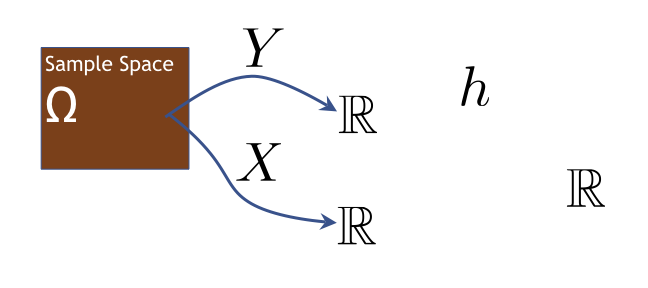
\includegraphics[width = .9\linewidth]{images/conditional_lotus}
       \begin{itemize}
\item Condition on $X=x$.
\end{itemize}
\note[item]{What about that famous rule that we called LOTUS?}
\note[item]{Remember what that was about.  if we have a random variable Y, and we pass it into a function h, that creates a new variable and we have a really nice formula for computing its expectation.}
       \note[item]{Is there a conditional version of this?  Yes!  Let's add R.V. $X$}
       \note[item]{If we condition on X, that's no problem, we just replace the distribution of Y with the conditional distribution, and plug it into LOTUS.}
       \note[item]{Here's an extra little wrinkle though: the theorem you see in the book is a little more powerful than this.  It turns out that we can make h depend on both X and Y.  that sounds really complicated, but it actually doesnt' change much.}
       \note[item]{When we condition on x, we treat X as a constant.  so h is essentially still just a function of Y.}

\end{frame}




\begin{frame}
 % \frametitle{Conditional Law of the Unthinking Statistician}
  
  \note[item]{And here's the full version of the conditional LOTUS. }
    \note[item]{The main thing to notice is that the equations look almost the same as before}
    \note[item]{we now have the conditional distribution instead of the regular distribution.}
    \note[item]{also, h can depend on y, but that doesn't change much because we've conditioned on y, so we can treat it as a constant.}
  
  \begin{block}{Theorem: Conditional LOTUS}
  Given discrete random variables $X$ and $Y$ with joint pmf $f$, and $h:\R^2 \rightarrow \R$,
$$  \E\big[h(X,Y) \big| X=x \big] = \sum_y h(x,y)f_{Y|X}(y|x),$$
For all $ x \in \text{Supp}[X]. $

  Given continuous random variables $X$ and $Y$ with joint pdf $f$, 
  $$  \E\big[h(X,Y) \big| X=x \big] = \int_{x=-\infty}^\infty h(x,y)f_{Y|X}(y|x)dy, $$
  for all $ x \in \text{Supp}[X].$
  \end{block}
  
  
\end{frame}


\begin{frame}
  %\frametitle{Linearity of Conditional Expectations}
  
  \begin{block}{Theorem: Linearity of Conditional Expectation}
  Given random variables $X$ and $Y$ and $a,b \in \R$, then for all $x \in \text{Supp[X]}$,
    $$\E \big[ aY + b \big| X=x  \big]  = a\E\big[ Y \big| X=x \big] + b$$
Moreover, given $g,h:\R \rightarrow \R$, then for all $x \in \text{Supp[X]}$,
  $$\E \big[ g(X)Y + h(X) \big| X=x  \big]  = g(x)\E\big[ Y \big| X=x \big] + h(x)$$
  \end{block}
\end{frame}



\begin{frame}
  \frametitle{Conditional Expectation Example}
  Simplify: $\E[ XY | X=x]$
\end{frame}



 
 \section{Demonstration of the Conditional Expectation Function}
 
 \begin{frame}
   \frametitle{Demonstration of the CEF}
   \textbf{Note: This is a Lecture and Software Demo, we're just
     placing it here for organization.}  \note[item]{Show the Plots of
     Marin Headlands rendered by Plotly.}  
   \note[item]{Notice that when we're at any particular X value, we
     have a whole function for the distribution of Y. This is the
     conditional pdf.}
   \note[item]{There is \textit{a lot} of information in this
     function.}
 \end{frame}
 
  \section{Reading: Conditional Expectation Function}

 \begin{frame}
   \frametitle{Reading: Conditional Expectation Function}
   \note[item]{We're going to make acoupld of notes for you, so grab
     your book and a pen (if you write in your books)}
   \begin{itemize}
   \item Read the second half of page 69, through page 71, stopping before the Law of Iterated Expectations.
     % \item \paul{switching to the function view seems like a big
     %   turn,
     %   maybe save that reading till we make the jump?}
   \item These pages are tough, so we're going to whiteboard
     theorems 2.2.11 and 2.2.12 on the other side of your reading.
   \item You can probably skip theorem 2.2.14 without great problem.
   \item Focus specific attention on definition 2.2.15.
   \end{itemize}
   \note[item]{Pay particular attention to definition 2.2.15 -- this
     is the pivot from the operator to the function, which has a lot
     more information. The notation here can be unclear -- it isn't
     your fault.}
 \end{frame}
 
 
 \section{Learnosity: Write a Conditional Expectation Function}
 
 \section{Introduction to the Law of Iterated Expectations}

 \begin{frame}
   \frametitle{Law of Iterated Expectations}
   Earlier, we worked with \textbf{theorem 1.1.13}, \textit{The law of
     total probability}, which stated:
   
   \begin{block}{Theorem 1.1.13: the law of total probability}
     If $\{A_{1}, A_{2}, A_{3}, \dots\}$ partition $\Sigma$,
     $B \in S$, and $P(A_{i}) > 0, \forall i$ then:
     \[
       P(B) = \sum_{i} P(B|A_{i})P(A_{i})
     \]
   \end{block}
   \begin{itemize}
   \item Useful because we can break the overall probability into
     smaller ``chunks'' whose probabilities might be easier to know. 
   \item The Law of Iterated Expectations is a generalization and reapplication
     of this principle.
   \end{itemize} 
 \end{frame}

 \section{Reading: Law of Iterated Expectations and Total Variance}

 \begin{frame}
   \frametitle{Reading: Law of Iterated Expectations}
   Read pages 72, 73, and the top of 74, stopping before theorem 2.2.19.
 \end{frame}

\section{Lightboard: Law of Iterated Expectations} 
 
\begin{frame}
  \frametitle{Law of Iterated Expectations}
  \note[item]{Check out 4.14 law of iterated expectations.  It
      does this in the first half, then there are two examples.  I'm
      cringing now, because I inappropriately assumed a binary gender.
      But perhaps we can just keep the first part before the examples.
      and film a separate ipad video with just one or two
      examples?}
  \note[item]{Why is this useful? Well, this says, if you can break
    down a statement into pieces, you can work them all back
    together. And, this is a continuous mapping version of the
    conditional probablity statement that we've seen earlier.}
  \note[item]{Because we're interested in conditional expectation
    functions, we're going to use this as a tool quite a bit through
    the rest of the course.}
\end{frame}

 \section{Law of Total Variance}

 \begin{frame}
   \frametitle{Splitting Variance}
   \note[item]{Remember when we started a few weeks ago from
     relatively simple axiomatic statements? We've built \textit{so
       much} since then! And, we've built it upon a foundation that we
     can know is solid, because we've deduced every
     piece.}  
   \note[item]{This is the last piece of tooling that we're going to
     build for this week. In the next sections we're going to apply
     this tooling against the BP and BLP.} 
   \note[item]{But, rather happily, this final piece of tooling itself
     has use -- splitting variance!}

   \begin{block}{Theorem 2.2.18: the law of total variance}
     For random variables $X$ and $Y$:
     \[
       \V[Y] = \V\big[\E[Y|X]\big] + \E\big[\V[Y|X]\big]
     \]
   \end{block}
   
   \textbf{Key question:} How much of the variance in $Y$ can be
   explained by $X$?
 \end{frame}
 
 \begin{frame}
   \frametitle{Splitting Variance: Example}
   $S$ represents salary.

   $O$ represents occupation (1 = data scientist, 2 = data engineer, 3
   = data analyst).  \note[item]{The law of total variance will work
     for any random variables, but it's easiest to understand if we
     condition on a discrete random variable}
   \begin{center}
     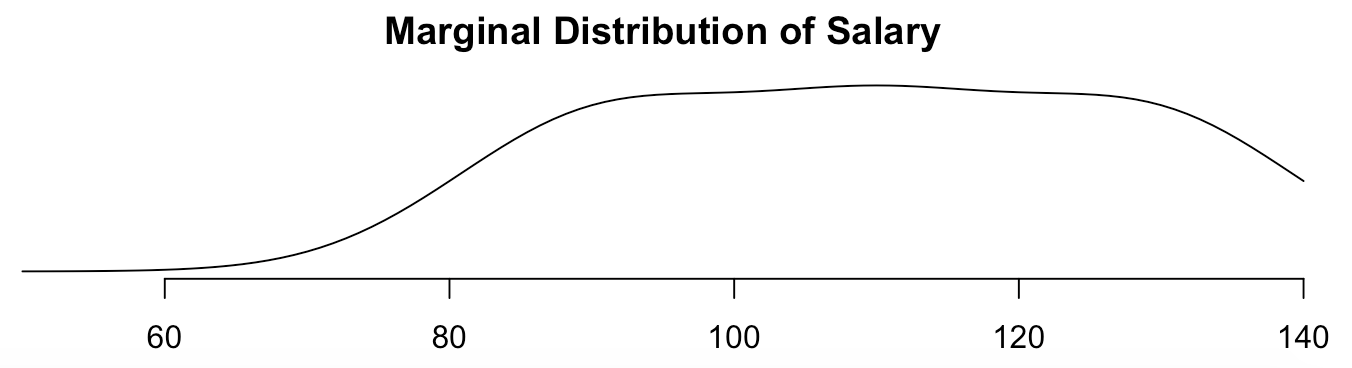
\includegraphics[width = 0.8\linewidth]{images/marginal_sal}
   \end{center}
   
   $\V[S] = 366$.  How much of this is explained by occupation?
 \end{frame}
 
 \begin{frame}
   \frametitle{Salary Conditioned on Occupation}
  
   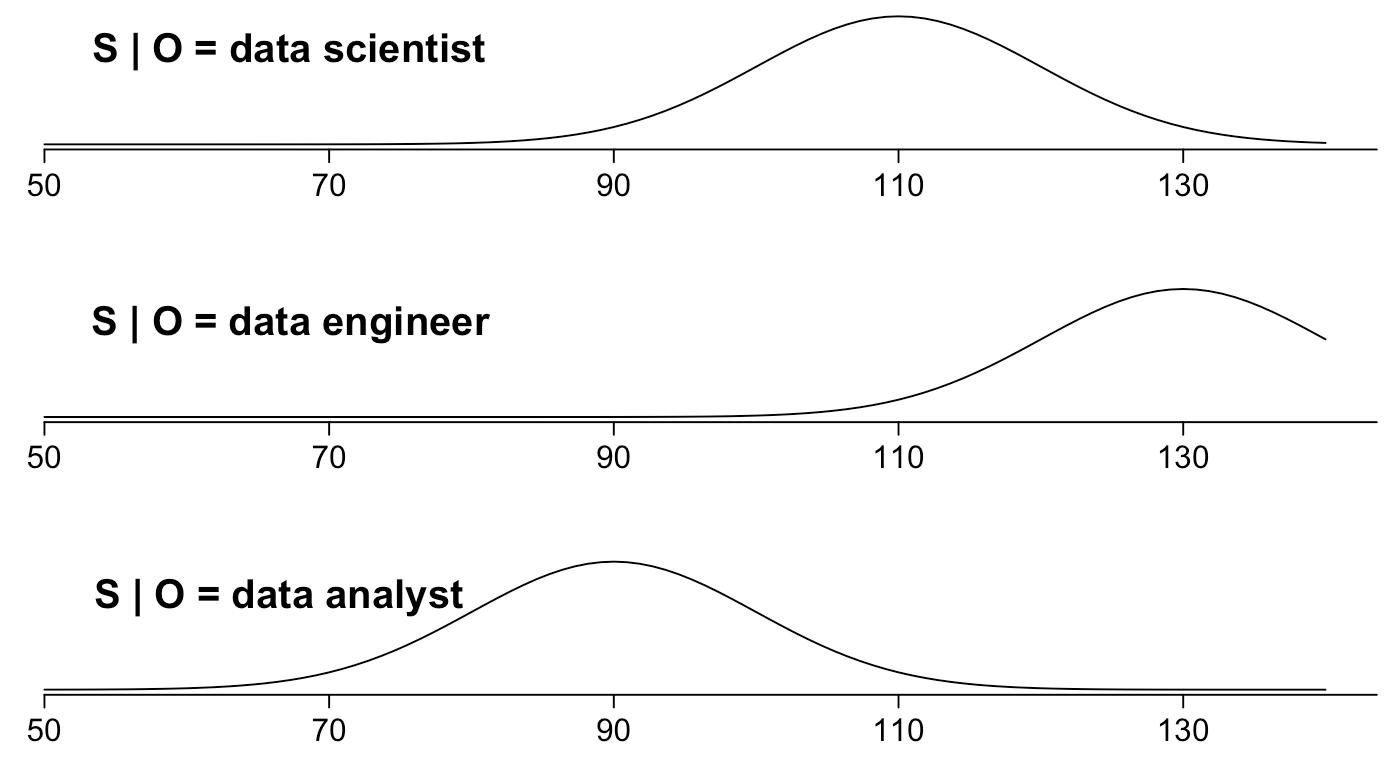
\includegraphics[width = \textwidth]{images/conditional_sal}

   \note[item]{Here we see the conditional distributions of S
       for different occupations.  For each one, we can mark $E(S|O)$,
       our best predictor for S once we observe O.}
   \note[item]{If these were all equal, then learning occupation
       doesn't help you make a prediction about salary.}
   \note[item]{The more the conditional expectation moves up and
       down - the more occupation gives us information about the
       salary} \note[item]{For each conditional distribution,
       we can also mark $V(S|O)$, the conditional variance of S once
       we observe O.}  \note[item]{The bigger these conditional
       variances, the more uncertainty there is in salary even after
       we observe occupation.}
 \end{frame}
 
 \begin{frame}
   \frametitle{Components of Variance}
   $\V[S]$ is the sum of two components.
   \begin{enumerate}
   \item \textbf{Explained variance:} $\V\big[\E[S|O]\big] = 266$
     \begin{itemize}
     \item Measures how much information $O$ gives about $S$
     \item Can also be called systematic variance
     \end{itemize}
     \note[item]{First we have $V\big[E[Y|X]\big]$.  This is the
       explained variance.  You can also call it the systematic
       variance or model variance. }

     \pause

   \item \textbf{Unexplained variance: $E\big[V[S|O]\big]=100$}
     \begin{itemize}
     \item Measures how much extra variation is there in $S$ that we
       can't explain with $O$
     \item Can also be called error variance
     \end{itemize}
     \note[item]{We may call this error variance, because we're really
       building a model for salary using occupation.  So if you tell
       me occupation, I use the model to give you an estimate for
       salary, but this is the uncertainty that's left over at the end
       - that's why we think of it as error.}
   \end{enumerate}
 \end{frame}

 \begin{frame}
   \frametitle{Law of Total Variance Implications}
   Suppose that you can divide data into groups along (possibly) two
   dimensions.
   \begin{enumerate}
   \item A dimension that does not explain any variation in outcomes
   \item A dimension that explains variation in outcomes
   \end{enumerate}

   As you're going to see in the next coding exercise, through this
   identity, if you can produce groups that have different means, you
   will necessarily produce a smaller $\E\big[\V[Y|X]\big]$.
 \end{frame}

 \section{Learnosity: Variance Breakdown}

 \begin{frame}
   \frametitle{Learnosity: Variance Breakdown}
   \textbf{Note: This is a learnosity activity. We're just including
     it here for organization.}

   \note[item]{Here we will ask students to work the code about
     temperature and pollution that we've written.} 
 \end{frame}

  \section{Best Predictors}
 \section{Deviations From the CEF}
 
 \begin{frame}
  \frametitle{More Comments for Alex}
  \note[item]{\paul{
      If you start with these plots in part 2 to describe what the CEF is
      (which I'm recommending), then you can use this space to bring them
      back and draw what epsilon is on them.}}
    \note[item]{
      For the proof that CEF minimizes MSE, I think you should first point
      out that this \textit{seems} easy.  We already proved that the mean
      minimizes MSE for one random variable.  so intuitively, you're taking
      the mean for every possible x.  In fact, the student might think (as I
      did earlier) that you can just take a first order condition for every
      x and be done.  But it doesn't work like that, because you can always
      choose some measure zero set of x's and alter their values without
      affecting MSE.  So the proof in the book is a clever way to avoid this
      and just show that CEF is one of the functions that minimizes MSE. 
    }
\end{frame}


\begin{frame}
  \frametitle{Joint Density Function}
  \note[item]{In this segment of learning, we're going to talk about
    the Conditional Expectation Function as a quantity of interest.}
  \note[item]{We'll begin by defining a quantity $\epsilon$ that is
    the difference between some particular value of $Y$ and what the
    CEF predict $E[Y|X]$.}  \note[item]{This error will be presented
    here, and we'll prove several features about $\epsilon$ that arise
    from the CEF. We'll also see this concept come back when we talk
    about regression in several weeks.}
  \note[item]{Once again, the distinction between an operator and a
    function is going to be important to keep in mind.} 

   For this section, we will work first with the same joint
   distribution function throughout.

   \begin{align*} 
     X & \sim U(min = 0, max = 10) \\
     W & \sim N(mean = 0, sd = 1) \\
     Y &= 10 - 2\cdot X + W
   \end{align*}

   \note[item]{Notice that here we're providing you the ``diety-eye''
     view. We don't get issued this, and we don't know how to estimate
     these functional forms yet. That will be the focus of the next
     section.} 
   Where $X$ and $W$ are independent.
   % \note[item]{ What can we \textit{know} about each of these
   % measurements
   % that I take?}
 \end{frame}

 \begin{frame}
   \frametitle{Joint Density Function (cont.)}
   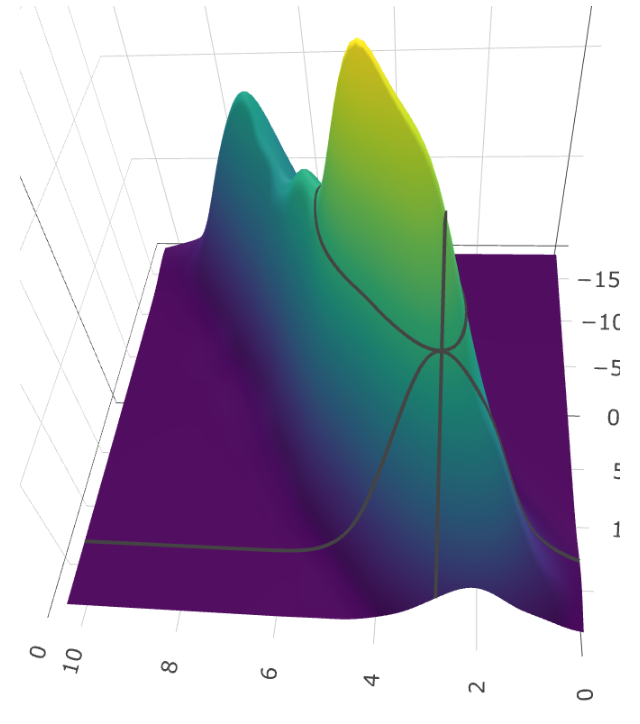
\includegraphics[width=0.49\linewidth]{images/marin_1}
   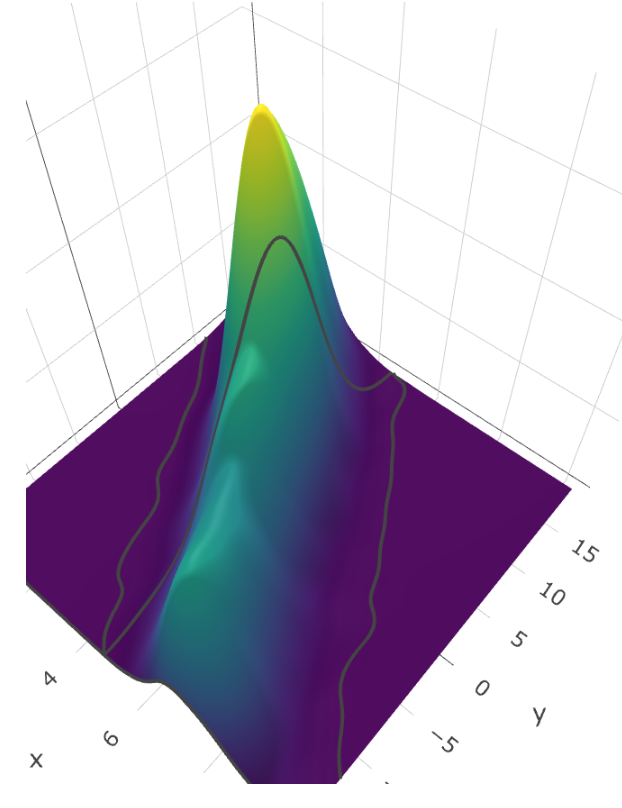
\includegraphics[width=0.49\linewidth]{images/marin_2}

   \note[item]{I like to think about this in terms of a probability
     landscape -- this is a simple one that has a single most probable
     set of outcomes. In general, this is not the case.} 
   \note[item]{Callout to the workbook that makes this plot.}
   \note[item]{Ask students to rotate the image so that they have made
     the plot and that the x axis ranges from 0 on the left, and 10 on
     the right; the y axis from -15 on the furthest to 15 on the
     nearest.} 
 \end{frame}

 \begin{frame}
   \frametitle{Deviations from the CEF}
   \begin{block}{Deviations from the CEF}
     Suppose that $\epsilon = Y - \E[Y|X]$ is the distance between my
     estimate within a grid and the actual value.  \note[item]{Notice
       that $Y$ is the actual continuous elevation that is modeled by
       the function of X and Y, but that $\E[Y|X]$ is the function that
       maps the CEF at the point $X=x$}
     \begin{itemize}
     \item Inside each of the grids, how far, on average, will I be from
       the true elevation? $\E[\epsilon|X] = ? $
     \item Across the whole ridgeline, how far, on average, will I be
       from the true elevation? $\E[\epsilon] = \E[\E[\epsilon?|X]] = $?
     \item Within each of the grids, what features will shape how
       close you are, on average? $\V[\epsilon | X] = ?$
     \item Across the whole ridgeline, what features will shape how
       close you are, on average? $\V[\epsilon] = ? $
     \end{itemize}
   \end{block}
 \end{frame}

\section{Reading: Deviations from the CEF}
 
 \begin{frame}
   \frametitle{Deviations from the CEF}
   \begin{itemize}
   \item Begin by reading from where we left off previously on page 74
     to the middle of page 76, stopping when the discussion turns to
     linear restrictions.
   \item Try to work through, on your own, the proof of why the CEF is
     the best (minimum MSE) estimator of Y.
   \item In the proof of theorem 2.2.20, the authors add
     $\E[\epsilon | X]$ seemingly from nowhere. This is a legal move
     because in 2.2.19, you have derived that $\E[\epsilon | X] = 0$.
   \end{itemize}
 \end{frame}

\section{Best Predictors}

\begin{frame}
  \frametitle{Predictors are Functions}
  
  \begin{block}{Definition: Predictor}
  Given random variables $X$ and $Y$, a predictor for $Y$ is a function, $g:\R \rightarrow \R$, such that $g(X)$ is regarded as a guess for $Y$.
\end{block}

\note[item]{Remember that Y is a random variable, and even if we condition on X, it still have a conditional distribution.}
\note[item]{But we want to represent that distribution with a single number.}

\begin{itemize}
\item Given a value $X=x$, a predictor suggests a single value for $Y$.
\item Define error as $\epsilon = Y - g(X)$.
\end{itemize}

\end{frame}


\begin{frame}
  \frametitle{Predictors and Errors}
     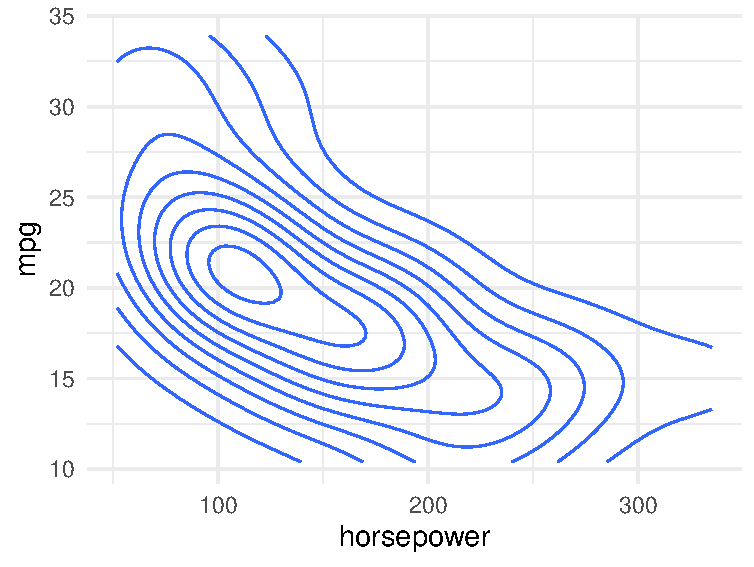
\includegraphics[width=\linewidth]{images/mpg}
     
     \note[item]{Let's see an example.  Here is a joint distribution, x is hp, y is mpg.}
     \note[item]{This is actually an estimated distribution, but let's pretend it's the real one.}
     \note[item]{A predictor for mpg is a function.  I'll draw one.}
     \note[item]{what happens if we take a draw from this distribution?}
     \note[item]{Nature reaches in and chooses a point.}
     \note[item]{Here is the predicted Y, and this distance is the error.}
     \note[item]{The predictor I drew is not a very good predictor.  what makes a good predictor?}
     \note[item]{We want the error to be small, but how do we do that?}
\end{frame}

\begin{frame}
  \frametitle{Choosing a Good Predictor}
  \note[item]{remember when we had one random variable, we discovered that the mean was the value that minimized expected squared error.}
  \note[item]{We can do the same thing here!}
\center
\textbf{Idea:} Minimize mean squared error, $\E[\epsilon^2]$.

\note[item]{By minimizing expected squared error, we'll be generalizing the mean, and we should end up with a function that stays close to the high probability areas.}
\end{frame}


\begin{frame}
\note[item]{So what do we get if we minimize MSE?  The answer is exactly the CEF!}
\note[item]{If you care about MSE, and you want to generate predictions of $Y$, you can't do any better than the CEF.}
\note[item]{This is a really important result.  It tells us what the maximum possible performance is for any predictor.}
\note[item]{And it helps us to view the CEF from an optimization perspective.  That's a viewpoint that really important in both classical statistics and machine learning.}
  \frametitle{Importance of the CEF}
  \begin{block}{Theorem: The CEF Minimizes MSE}
  Given random variables $X$ and $Y$, the CEF $\E[Y|X]$ has the smallest MSE out of all predictors of $Y$.
  \end{block}
\end{frame}




%
%\section{Drawing the CEF}
% 
% \begin{frame}
%   \frametitle{Drawing the CEF}
%   \centering
%   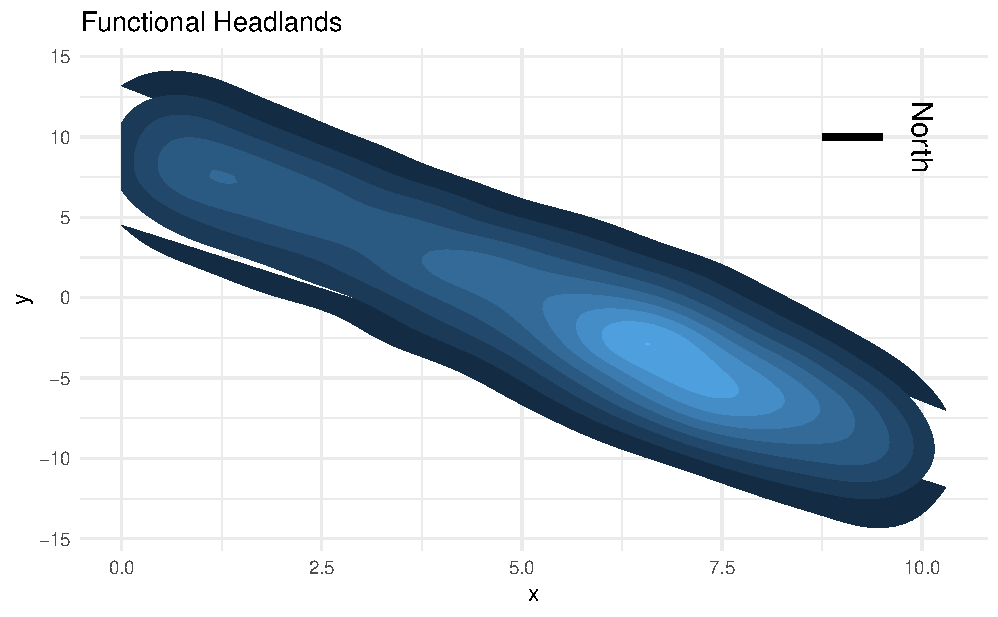
\includegraphics[width=\linewidth]{./images/marin_density.pdf}
%   \note[item]{\alex{Paul, let's revisit the complexity of this
%       function. You're convincing me that perhaps this could be more
%       complex to keep from confusing students.} Let's see if we can
%     generate a simple functional form that we can work with --
%     polynomial degree 2?} 
%   \note[item]{Let's return to the joint density plot but
%     now we will represent it in two dimensions, rather than three.}
%   \note[item]{We have the same goal, understanding the height of the probability.}
%   \note[item]{Here we will take some ink off the paper, so that we
%     can draw more clearly.} 
% \end{frame}
%
%\begin{frame}
%  \frametitle{Drawing the CEF (cont.)}
%  \centering
%  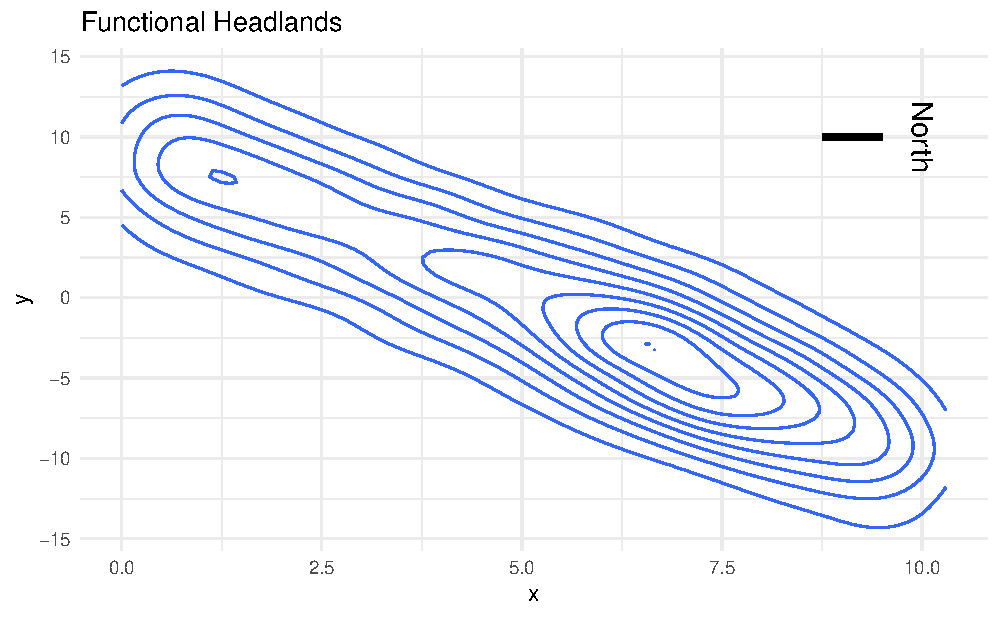
\includegraphics[width=\linewidth]{./images/marin_contour.pdf}
%  \note[item]{Let's return to the plot that we've made of Marin, but
%    now we will represent it in two dimensions, rather than three.}
%  \note[item]{We have the same goal, understanding the height of the
%    mountain.}
%  \note[item]{Here we will take some ink off the paper, so that we
%    can draw more clearly.} 
%\end{frame}
%
% \begin{frame}
%   \frametitle{Drawing the CEF (cont.)}
%   \centering
%   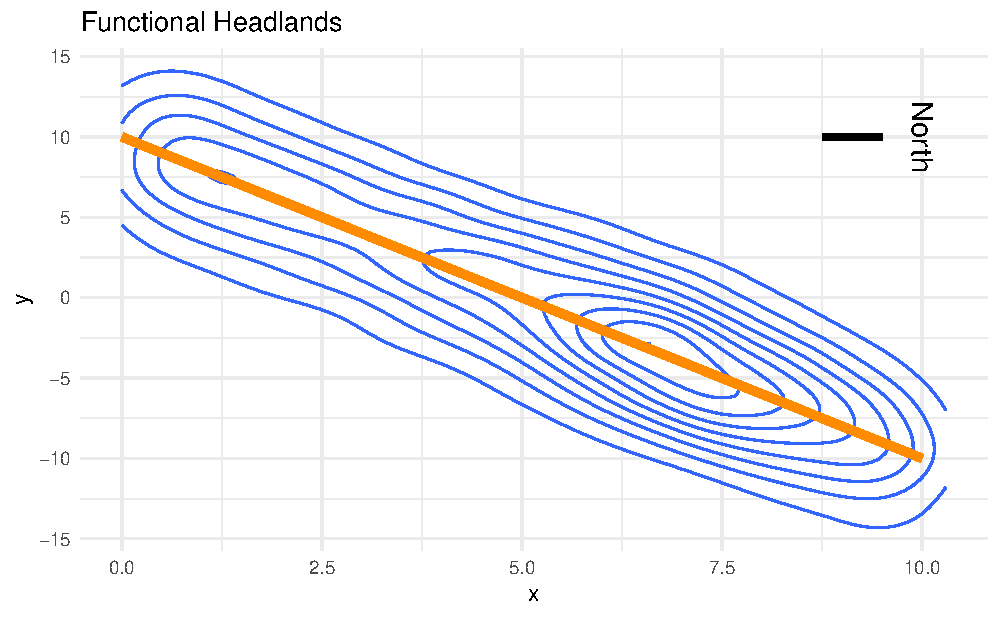
\includegraphics[width=\linewidth]{./images/marin_contour_highest_prob.pdf}
% \end{frame}
%
% \begin{frame}
%   \frametitle{Implications of Knowing the CEF}
%   \begin{itemize}
%   \item If we can produce a statement about the CEF, we can produce
%     the \textit{best} estimates possible about the target outcome,
%     given values of X.
%   \item Just as the $\E[Y]$ is the best (smallest MSE) estimate of $Y$,
%     $\E[Y|X]$ is the best (also smallest MSE) estimate of $Y$, given
%     information about $X$.
%   \end{itemize}
% \end{frame}
%
%\section{Learnosity: Produce the CEF}
%
% \begin{frame}
%   \frametitle{Working to Know the CEF}
%      \begin{block}{Marin setup}
%     \begin{align*}
%       X & \sim U(0, 10) \\
%       W & \sim N(0, 3) \\
%       Y & = 10 - 2\cdot X + W \\
%       & X \Perp W \\ 
%       \E[X] & = 
%     \end{align*}
%   \end{block}
%   \begin{enumerate}
%   \item Produce the conditional expectation function, $G_{Y}(x) =
%     \E[Y|X]$.
%   \end{enumerate}
%   \note[item]{\paul{This would feel more like a foundational exercise if you provided just the joint pdf.}}
% \end{frame}

\section{Lightboard: The CEF Minimizes MSE}

\begin{frame}
  \frametitle{The CEF minimizes MSE}
    \hspace{-1.2cm} 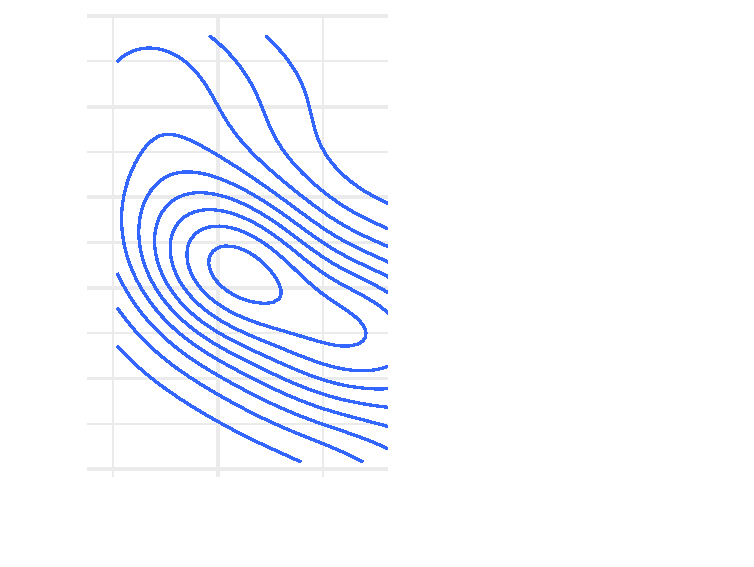
\includegraphics[width=.5\linewidth]{images/mpg_narrow}
     \note[item]{draw the CEF $E[Y|X]$, and draw some other predictor, $g(X)$.}
     \note[item]{Let's let $W$ be the distance between these two lines.  $W= \E[Y|X] - g(X)$.  technically, W is a random variable, but it's a function of X so it's just a number if we look at a specific X.}
     \note[item]{We want to show that any distance $W$ makes the MSE worse.}
     \note[item]{write the error: $Y-g(x) = Y - E(Y|X) + E(Y|X) - g(X) = \epsilon + W$}
     \note[item]{Look at the conditional expectation: $E[ (Y - g(X))^2 | X] = E[ (\epsilon + W)^2 | X] = E[ \epsilon^2 + 2 \epsilon W + W^2 | X] = E[\epsilon^2 | X] + 2W E[ \epsilon | X] + W^2$}
     \note[item]{We know $E[\epsilon|X] = 0$ so the middle term disappears.}
          \note[item]{We can use law of iterated expectations on MSE: $MSE = E[ E[ (Y - g(X))^2 | X] ] = E[ E[\epsilon^2 | X] + W^2]  = E[\epsilon^2] + E[W^2] \geq E[\epsilon^2] $}
         
\end{frame}


 \section{Best Linear Predictors} 
 
 \begin{frame}
  \frametitle{Complexity of the CEF}
  \note[item]{Think about the CEF as a model for some random variable - mpg in this case.}
  \note[item]{It's a good model in one sense - it minimizes MSE}
  \note[item]{Bit the CEF can be quite complicated.  It takes an infinite number of numbers to specify the CEF.}
  \note[item]{If you had all that information, how would you use it?}
  \note[item]{Can you reason about every detail in this curve?}
  \note[item]{Can you communicate what you see? Can you compare your results against another researcher's?}
  \note[item]{The fact is, even if we could estimate the CEF (which takes a LOT of data), we're not well equipped to analyze it directly.}
  \note[item]{So you actually don't find too many analyses that estimate the CEF.}
   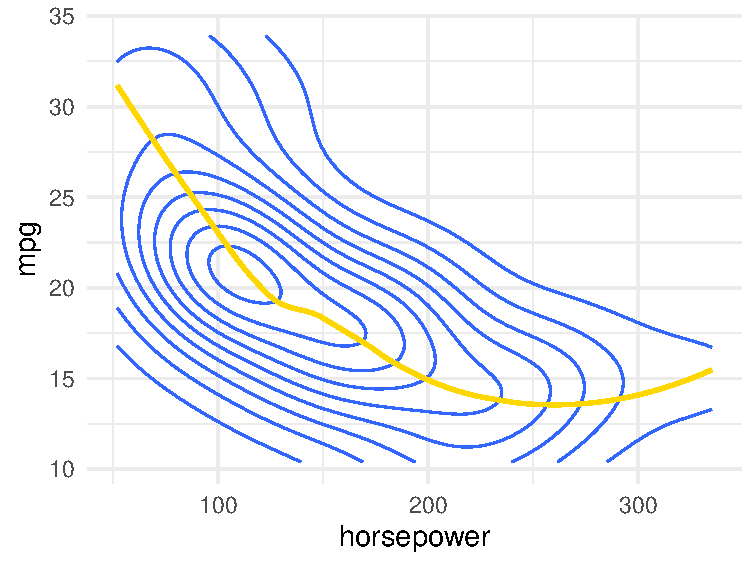
\includegraphics[width=\linewidth]{images/mpg_cef}
\end{frame}


\begin{frame}
  \frametitle{Linearizing the Predictor}
  \note[item]{This tells us that we need a simpler model.  The simplest possible model that captures a relationship: a line.}
  \note[item]{This is what we call a linear predictor.}
  \note[item]{There are some disadvantages to using a linear predictor.}
  \note[item]{The joint distribution many not look especially linear.  We're covering up a lot of complexity.}
  \note[item]{Except for very artificial situations, a linear predictor will have worse MSE than the CEF.}
  \note[item]{But there are some major advantages.}
  \note[item]{You only need a few numbers to write down a linear predictor - the slope is most important.}
  \note[item]{The slope is easy to communicate, you can compare studies against each other.}
  \note[item]{You have a single number that captures an overall relationship.}
     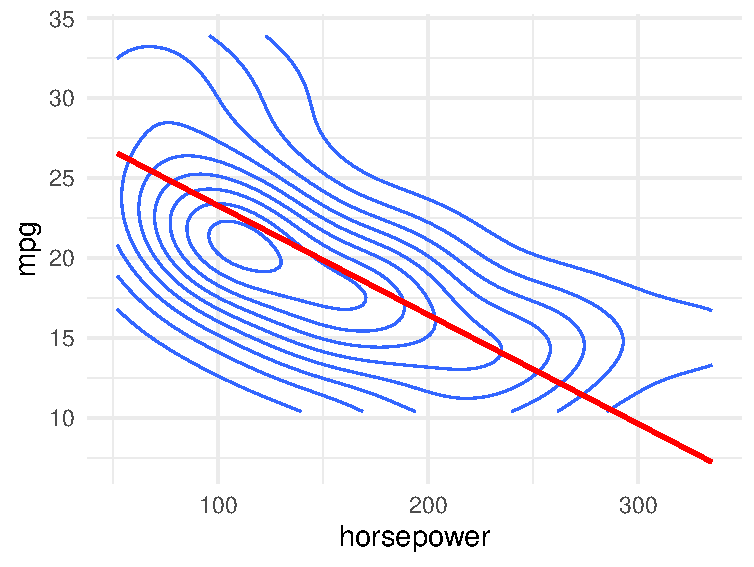
\includegraphics[width=\linewidth]{images/mpg_lm}
\end{frame}


\begin{frame}
  \frametitle{Choosing a Linear Predictor}
  \note[item]{How do you choose a linear predictor?}
  \note[item]{There are different strategies, so it depends on your goals}
  \note[item]{But the most common idea is to continue our previous strategy, make MSE as small as possible.}
  \note[item]{Read definition}
  
  \begin{block}{Definition: The Best Linear Predictor (BLP)}
  Given random variables $X$ and $Y$, the \textit{best linear predictor (BLP)} for $Y$ is the function $g:\R \rightarrow \R$, $g(X) = \alpha + \beta X$, with coefficients given by,
  
 $$ \text{argmin}_{\alpha, \beta} \E\Big[ \big( Y - (\alpha + \beta X) \big)^2 \Big]$$
  \end{block}
\end{frame}



\begin{frame}
  \frametitle{Solving for the BLP}
  \note[item]{Here's another reason to use the Best Linear Predictor.}
  \note[item]{You can solve for the coefficients that minimize MSE, and they have a really elegant solution.}
  \note[item]{Remember this form for the slope: it's a covariance over a variance.}
  \begin{block}{Theorem: The BLP Solution}
  Given random variables $X$ and $Y$, the best linear predictor for $Y$ is given by $g(X) = \alpha + \beta X$, where,
  
  $$\beta = \frac{\cov[X,Y]}{\V[X]}, \qquad \alpha = \E[Y] - \frac{\cov[X,Y]}{\V[X]}\E[X]$$
  \end{block}
\end{frame}






  
%  \begin{frame}
%   \frametitle{Why Linearize?}
%   \note[item]{A clear limitation is that this this joint CDF can be
%     complicated.}
%   \note[item]{If we had to do this work, by hand we would be in
%     trouble.}
%   \note[item]{But, the knottyness of working with these joint
%     densities is reflected in the difficulty in the data science
%     space as well -- these functions are unknown, and even if they
%     \textit{were} known, they might not have nice properties.} 
%   \begin{itemize}
%   \item What if we wanted to restrict our statement about the CEF
%     to a \textit{simpler} representation? Simple enough that we could
%     describe the function by a line?
%     \note[item]{Notice that as soon as we talk about linear
%       dependence, you should be thinking back to the covariance and
%       correlation sections from earlier.}
%   \item Then, as the reading on page 76 to the top of page 79 demonstrates, we can
%     produce the best (lowest MSE) variant of this line using
%     $\V[\cdot]$ and $\text{\cov}[\cdot, \cdot]$ operators that we
%     have developed!
%   \item Suppose the line has some intercept $\alpha$ that is 
%     $\E[Y|X=0]$ and some slope $\beta$ that characterizes how the
%     outcome changes as X changes. 
%   \end{itemize} 
% \end{frame}
 
 \section{Reading: The Best Linear Predictor}
 
 \begin{frame}
   \frametitle{Reading Assignment: Linear Approximation}
   
   Read to the middle of page 79, stopping before you get to example
   2.2.23. \note[item]{This is why we have avoided paramterizing the
     random variables $X$ and $Y$ to this point. Performing these
     integrations can be tedious, but does highlight the process of
     applying the expectation operator.} 
   \end{frame}
   
   \section{Moment Conditions}
   
   \begin{frame}[t]
  \frametitle{Moment Conditions}
  The BLP is given by  $\text{argmin}_{\alpha, \beta} \E\Big[ \big( Y - (\alpha + \beta X) \big)^2 \Big]$
\end{frame}


  \begin{frame}[t]
  \frametitle{Moment Conditions - Solution}
  The BLP is given by  $\text{argmin}_{\alpha, \beta} \E\Big[ \big( Y - (\alpha + \beta X) \big)^2 \Big]$
  \note[item]{If you put in different values of $\alpha$ and $\beta$ you can get different value of the expectation - so think of it as a function of $\alpha$ and $\beta$. }
  \note[item]{How do you minimize a function?  you can use calculus, use your first order conditions.}

\note[item]{This next step is a little confusing.  it turns out that we can move the expectation outside of the derivative.  that's because the expecation is a sum or an intergral, so it passes through derivatives.}
\note[item]{What's happening here?  first, nature reaches in and chooses a data point, which defines an error.  then if you move $\alpha$, that error goes up or down and we can calculate a derivate.  but that depends on the point that was chosen, so it's a random variable.  and we take an expectation over all the possible points.}

$0 = \frac{\partial \E[\epsilon^2]}{\partial \alpha} = \E\left[ \frac{\partial \epsilon^2}{\partial \alpha}   \right] 
= \E\left[  2\epsilon \frac{\partial \epsilon}{\partial \alpha}   \right] = -2 \E[\epsilon]$

 $0 = \frac{\partial \E[\epsilon^2]}{\partial \beta}  = \E\left[ \frac{\partial \epsilon^2}{\partial \beta}   \right] 
= \E\left[  2\epsilon \frac{\partial \epsilon}{\partial \beta}   \right] = -2 \E[\epsilon X]$

Version 1:
\begin{enumerate}
\item $\E[\epsilon] = 0$
\item $\E[\epsilon X] = 0$
\end{enumerate}

Version 2:
\begin{enumerate}
\item $\E[\epsilon] = 0$
\item $cov[\epsilon, X] = \E[\epsilon X] - \E[\epsilon]\E[X] = 0$
\end{enumerate}

What about $\E[\epsilon | X]$?

\note[item]{It turn out that not only does the BLP fulfill the moment conditions, it's the ONLY line that does.  I'm not going to show it, but you can check all the derivatives to see that the MSE has one minimum.}
\end{frame}

\section{Lightboard: Understanding Moment Conditions}

\begin{frame}
  \frametitle{Understanding Moment Conditions}
 \begin{enumerate}
 \item $0 = \E[\epsilon]$
\item $0 = \cov[\epsilon, X]$
\end{enumerate}
  \hspace{-1cm} 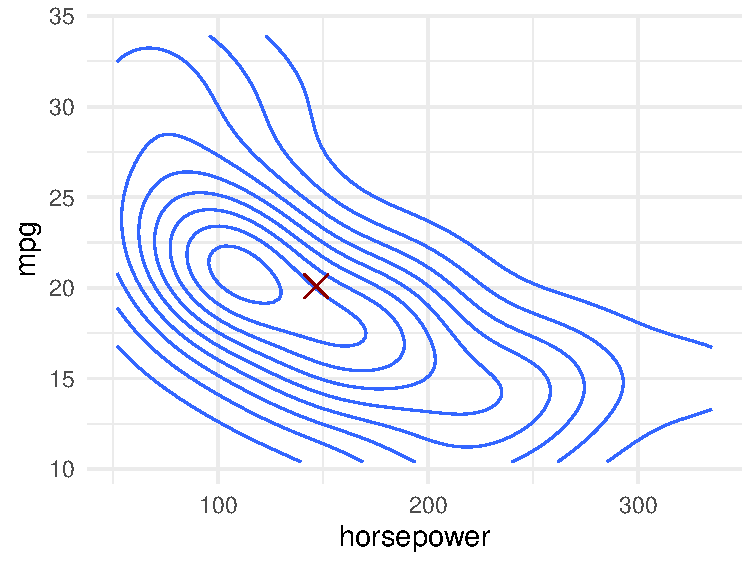
\includegraphics[width=.8\linewidth]{images/mpg_mean}

\note[item]{Here is a way to think about the moment conditions that I find useful}
\note[item]{Say you want to choose a linear predictor.  at first, you're considering every possible line through this plane.}
\note[item]{Now impose the first moment condition.  this tells us our line passes through this point.  but that's still many different lines.  how do we choose one?}
\note[item]{Let's draw one and see what happens.  For this line, when X is high, the error tends to be negative. when x is low, the error tends to be positive.  so the cov is negative.}
\note[item]{$cov[\epsilon,X] < 0 \implies$ slope too high.}
\note[item]{$cov[\epsilon,X] > 0 \implies$ slope too low.}
\end{frame}

\begin{frame}
  \frametitle{Understanding Moment Conditions - Solution}
  \begin{enumerate}
\item $0 = \E[\epsilon] = \E \left[ Y - (\alpha + \beta X) \right] \implies \E[Y] = \alpha + \beta \E[X]$
\item $0 = \cov[\epsilon, X]$
\end{enumerate}
  \hspace{-1cm} 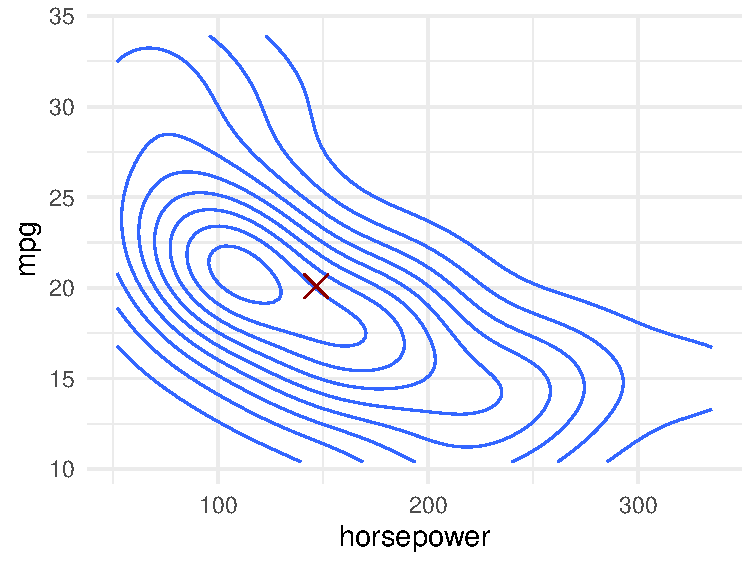
\includegraphics[width=.8\linewidth]{images/mpg_mean}

\note[item]{Here is a way to think about the moment conditions that I find useful}
\note[item]{Say you want to choose a linear predictor.  at first, you're considering every possible line through this plane.}
\note[item]{Now impose the first moment condition.  this tells us our line passes through this point.  but that's still many different lines.  how do we choose one?}
\note[item]{Let's draw one and see what happens.  For this line, when X is high, the error tends to be negative. when x is low, the error tends to be positive.  so the cov is negative.}
\note[item]{$cov[\epsilon,X] < 0 \implies$ slope too high.}
\note[item]{$cov[\epsilon,X] > 0 \implies$ slope too low.}
\end{frame}


\section{Lightboard: The BLP Solution}

\begin{frame}[t]
  \frametitle{The BLP Solution}
  The BLP is defined by the moment conditions:
  \begin{enumerate}
  \setlength\itemsep{2.5em}
\item $0 = \E[\epsilon] $
\item $0 = \E[\epsilon X] $
\end{enumerate}
\end{frame}


\begin{frame}[t]
  \frametitle{The BLP Solution - Solution}
    The BLP is defined by the moment conditions:
  \begin{enumerate}
\item $0 = \E[\epsilon] = \E \left[ Y - (\alpha + \beta X) \right] = \E[Y] - \alpha - \beta \E[X]$. $\alpha =  \E[Y]  - \beta \E[X]$.
\item $0 = \E[\epsilon X] = \E \left[ \big( Y - (\alpha + \beta X) \big) X \right]  = \E[XY] - \alpha\E[X] - \beta \E[X^2] $
$ =  \E[XY] - \Big( \E[Y]  - \beta \E[X]\Big)\E[X] - \beta \E[X^2] $
$ =  \E[XY] -  \E[X]\E[Y]  + \beta \E[X]^2 - \beta \E[X^2] $
$ = \cov[X,Y] - \beta \V[X] $
\end{enumerate}

$\beta = \frac{\cov[X,Y]}{\V[X]}$

$\alpha = \E[Y] - \frac{\cov[X,Y]}{\V[X]} \E[X]$
\end{frame}



%
%   \begin{frame}
%     \frametitle{Characteristics of the BLP}
%     The BLP:
%     \begin{itemize}
%     \item Is a function of $X$, $g(X) = \alpha + \beta X$
%     \item Produces the smallest possible MSE of linear estimators
%     \item In some special cases, is equivalent to the CEF
%     \item In some cases, produces MSE that are similar to the CEF 
%     \item MSE performance depends on distribution of data, but BLP is
%       always the \textit{best} linear estimator
%     \end{itemize}
%   \end{frame}

\section{Reading: Multivariate Generalizations}

\begin{frame}
  \frametitle{Reading: Multivariate Generalizations}
  
  Read section 2.3, Multivariate Generalizations.
\end{frame}


\section{Best Linear Predictors in Higher Dimensions}

   \begin{frame}
     \frametitle{Linear Predictors in Higher Dimensions}
     \begin{block}{Definition: Linear Predictor}
Given random variable $Y$, and random vector $\bs{X} = (1, X_1, X_2, X_3,...,X_k)$

     
     A \textit{linear predictor} for $Y$ is a function, $g:\R^k \rightarrow \R$ of the form,
     $$g(x_0, x_1,x_2,...,x_k) = \beta_0 x_0 + \beta_1 x_1 + \beta_2 x_2 + ... + \beta_k x_k$$
     
      such that $\hat Y = g(1, X_1, X_2,...,X_k)$ is regarded as a guess for $Y$.
      
  \end{block}
   \end{frame}
   
   
\begin{frame}
  \frametitle{Interpreting Model Coefficients}
  
  \note[item]{How do we interpret the betas in a linear predictor?}
  \note[item]{This actually applies to any linear predictor, not just the best one.}
  \note[item]{To get an idea, try taking the partial derivative of the
    predicted outcome, with respect to some $X_i$} 
  \note[item]{This means that you can think of $\beta_i$ as the change
    in the outcome when $X_i$ changes by 1 unit, but the partial is
    very important.  This is ONLY true if the other $X$'s are held
    constant.}
  
  \begin{align*}
    \hat{Y} &=\beta_0 + \beta_1 X_1 + \beta_2 X_2 + ... + \beta_k X_k\\
    \frac{\partial \hat{Y}}{\partial X_i} &= \beta_i, \quad \ \  \Delta \hat{Y} = \beta_{i} \cdot \Delta X_{i}
  \end{align*}
     \begin{block}{   \textbf{Ceteris Paribus:} All else equal}
    \begin{itemize}
    \item If $X_{i}$ changes by $\Delta X_{i}$, the prediction $\hat{Y}$ changes by $\beta_{i} \cdot \Delta X_{i}$, \textit{if the other $X$'s are held constant}.
    \end{itemize} 
 
  \end{block} 
\end{frame}
  

\begin{frame}
  \frametitle{Interpreting Model Coefficients - Example}
 
  Does this model say peacocks with longer tails fly slower?  

  \[
    \widehat{\text{air\_speed}} = 4.3 - 1.2 \cdot \text{tail\_length} + 0.8
    \cdot \text{muscle\_mass}
  \]
 
 \centering
 \centering
 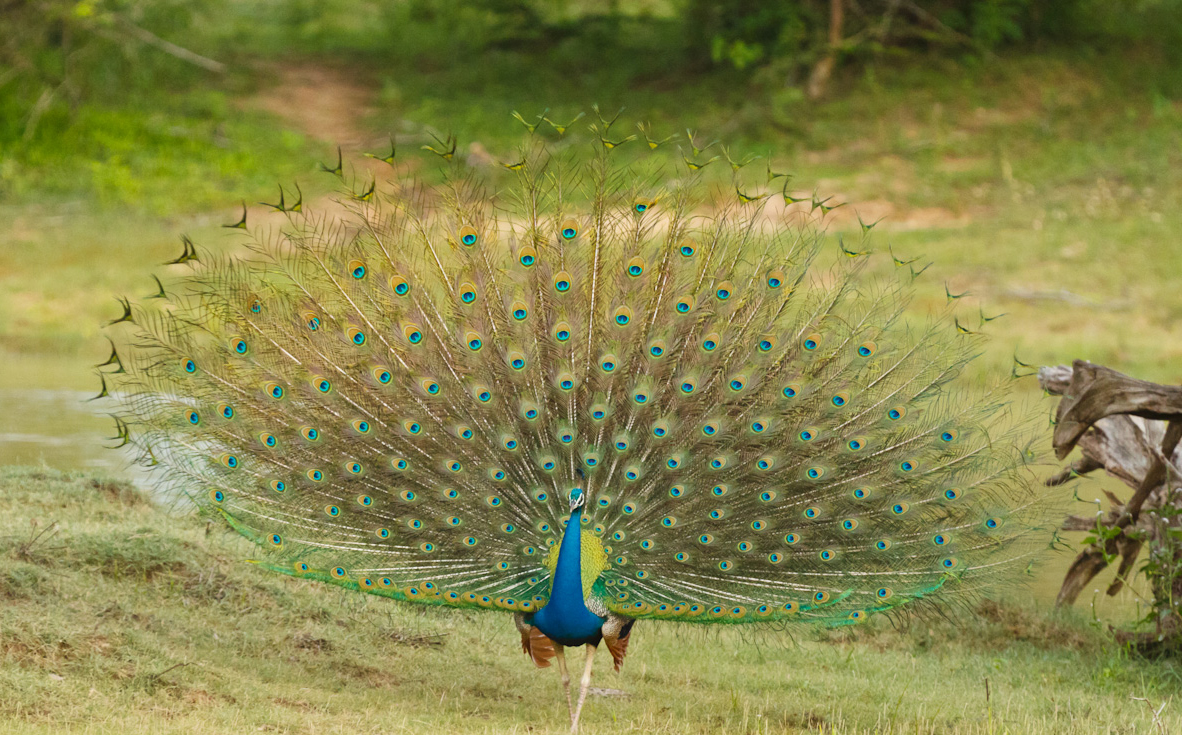
\includegraphics[width = .6 \textwidth]{images/peacock}\\
  \vspace{-.3cm} \scalebox{.5}{Photo by Thimindu Goonatillake CC BY-SA
    2.0}

  \note[item]{Here's a predictor that we developed to describe the flying
    speed of male peacocks.} 
  \note[item]{Notice the coefficient on the tail length variable: $-1.2$}
  \note[item]{Does this suggest that peacocks with longer tails are
    slower flyers?}  
  
  \note[item]{The answer is no - we have to remember ceteris paribus}
  \note[item]{The correct interpretation is that peacocks with1 unit
    longer tails, but the same muscle mass, are predicted to fly 1.2
    units slower.  But what about peacocks with longer tails as a
    whole?  We just don't know.  For example, peacocks with
    longer tails might also have more muscle mass.  Maybe they fly
    faster.} 
\end{frame}


    \begin{frame}
     \frametitle{Best Linear Predictors in Higher Dimensions}
     \begin{block}{Definition: Best Linear Predictor}
Given random variable $Y$, and random vector $\bs{X} = (1, X_1, X_2, X_3,...,X_k)$

     
     The \textit{best linear predictor} for $Y$ is the function, $g:\R^{k+1} \rightarrow \R$,
     $g(x_0 ,x_1,x_2,...,x_k) = \beta_0 x_0 + \beta_1 x_1 + \beta_2 x_2 + ... + \beta_k x_k$, with coefficients given by,
      $$ \text{argmin}_{\beta_0,...,\beta_k} \E\Big[ \big( Y - (\beta_0 + \beta_1 X_1 + ... + \beta_k X_k) \big)^2 \Big]$$

      
  \end{block}
   \end{frame}


\begin{frame}
  \frametitle{Moment Conditions in Higher Dimensions}
%  Let $\epsilon = Y - (\beta_0 + \beta_1 X_1 + ... + \beta_k X_k) \big)^2$
  Apply first-order conditions:
  
 $0 = \frac{\partial \E[\epsilon^2]}{\partial \beta_0} = \E\left[ \frac{\partial \epsilon^2}{\partial \beta_0}   \right] 
= \E\left[  2\epsilon \frac{\partial \epsilon}{\partial \beta_0}   \right] = -2 \E[\epsilon]$

For $j>0$, $0 = \frac{\partial \E[\epsilon^2]}{\partial \beta_j}  = \E\left[ \frac{\partial \epsilon^2}{\partial \beta_j}   \right] 
= \E\left[  2\epsilon \frac{\partial \epsilon}{\partial \beta_j}   \right] = -2 \E[\epsilon X_j]$

Version 1:
\begin{enumerate}
\item $\E[\epsilon] = 0$
\item $\E[\epsilon X_j] = 0$
\end{enumerate}

Version 2:
\begin{enumerate}
\item $\E[\epsilon] = 0$
\item $cov[\epsilon, X_j] = 0$
\end{enumerate}
\end{frame}


\begin{frame}
  \frametitle{The BLP Solution in Higher Dimensions}
  $$\bs{\beta} = \E\big[ (\bs X^T \bs X)^{-1} \big] \E\big[\bs X^TY\big]$$
  \note[item]{Finally, i just want to mention that there is a closed form solution to the BLP, even in higher dimensions.}
  \note[item]{This solution requires some matrix algebra, so we won't get into it now.}
  \note[item]{We'll come back later and talk about ordinary least squares regression, which is a technique for estimating the BLP, using a sample of data.}
  
\note[item]{  At that point, we'll spend more time explaining the matrix operations.}
\note[item]{For now, just remember that the BLP is a way to summarize the relationship among variables, and it's the target of interest for a lot of research.}
\end{frame}

\begin{frame}
  \frametitle{Looking Ahead}
\begin{itemize}
\item   The Best Linear Predictor is also called the Population Regression Function.
\item   Linear Regression: An algorithm for selecting a linear predictor given a sample of data.
\item  Ordinary Least Squares Regression: An algorithm for estimating the best linear predictor.
\note[item]{It's hard to overemphasize how important the BLP is. <read>}
\note[item]{This means that the BLP is really the core object of interest for a HUGE amount of research.}
\note[item]{So don't forget this -we'll have a lot more to say about it.}
\end{itemize}

\end{frame}

%
%   \begin{frame}
%     \frametitle{Turning Out to Vote}
%     Suppose that we can measure two attributes for
%     citizens: their age and their party ID. Then, we can produce
%     the \textit{best} (minimum MSE) estimate of the likelihood using
%     a conditional expectation within parties and across ages.
%   \end{frame}
%
%   \begin{frame}
%     \frametitle{Context in the Course}
%     \begin{itemize}
%     \item At this point, we have relied on random variables—functions 
%       that map real world events into the $\mathbb{R}$
%       space—and probability functions to produce summaries of
%       models. 
%     \item All of this has been done without data to derive
%       theoretical guarantees about how these functions and their
%       summaries behave.
%     \item In the next weeks of the course, we're going to build
%       sampling theory to know how these theoretical guarantees can
%       be informative when we have to \textit{fit} functions from data.
%     \end{itemize}
%   \end{frame}

\end{document}
